\chapter*{Anexo}

\section*{Cuestionario para Evaluar la Interpretabilidad de los Modelos}

El cuestionario incluye los siguientes tipos de preguntas:
\begin{itemize}
    \item Preguntas de Exactitud: Pedir al usuario que realice una predicción basada en el modelo.
    \item Preguntas de Detección de Error: Presentar al usuario una observación y una predicción realizada por el modelo y preguntar si es correcta.
    \item Métricas de Interpretabilidad Indirectas: Se incluirán métricas como el cuestionario NASA-TLX para evaluar la carga cognitiva y se medirá el tiempo utilizado por el usuario para responder cada pregunta.
\end{itemize}

Para garantizar una evaluación completa y detallada, se propone un cuestionario con un total de 20 preguntas:
\begin{itemize}
    \item 12 Preguntas de Exactitud:
    \begin{itemize}
        \item 6 preguntas resueltas por ambos modelos (DT e IDS).
        \item 3 preguntas ambiguas para evaluar la capacidad de manejo de incertidumbre.
        \item 3 preguntas exclusivas para cada modelo para destacar diferencias en la estructura y enfoque.
    \end{itemize}
    \item 8 Preguntas de Detección de Error:
    \begin{itemize}
        \item 4 preguntas resueltas por ambos modelos.
        \item 2 preguntas ambiguas para evaluar cómo los modelos manejan la incertidumbre y errores potenciales.
        \item 2 preguntas exclusivas para cada modelo.
    \end{itemize}
\end{itemize}

\subsection*{Preguntas de Exactitud}

\subsubsection*{Preguntas resueltas por ambos modelos}
\begin{itemize}
    \item Observación: \texttt{absences = 1, failures = 1, studytime = 2, age = 18}\\
    Predicción:
    \begin{itemize}
        \item a) Aprobado
        \item b) No aprobado
        \item c) No estoy seguro
    \end{itemize}
    Modelo: Ambos modelos predicen No Aprobado

    \item Observación: \texttt{absences = 4, failures = 0, studytime = 3, age = 16}\\
    Predicción:
    \begin{itemize}
        \item a) Aprobado
        \item b) No aprobado
        \item c) No estoy seguro
    \end{itemize}
    Modelo: Ambos modelos predicen No Aprobado

    \item Observación: \texttt{absences = 3, failures = 1, studytime = 1, age = 15}\\
    Predicción:
    \begin{itemize}
        \item a) Aprobado
        \item b) No aprobado
        \item c) No estoy seguro
    \end{itemize}
    Modelo: Ambos modelos predicen Aprobado

    \item Observación: \texttt{absences = 0, failures = 0, studytime = 1, age = 18}\\
    Predicción:
    \begin{itemize}
        \item a) Aprobado
        \item b) No aprobado
        \item c) No estoy seguro
    \end{itemize}
    Modelo: Ambos modelos predicen Aprobado

    \item Observación: \texttt{absences = 1, failures = 0, studytime = 2, age = 15}\\
    Predicción:
    \begin{itemize}
        \item a) Aprobado
        \item b) No aprobado
        \item c) No estoy seguro
    \end{itemize}
    Modelo: Ambos modelos predicen Aprobado

    \item Observación: \texttt{absences = 0, failures = 1, studytime = 3, age = 18}\\
    Predicción:
    \begin{itemize}
        \item a) Aprobado
        \item b) No aprobado
        \item c) No estoy seguro
    \end{itemize}
    Modelo: Ambos modelos predicen No Aprobado
\end{itemize}

\subsubsection*{Preguntas ambiguas}
\begin{itemize}
    \item Observación: \texttt{absences = 3, failures = 1, studytime = 2, age = 17}\\
    Predicción:
    \begin{itemize}
        \item a) Aprobado
        \item b) No aprobado
        \item c) No estoy seguro
    \end{itemize}
    Modelo: La combinación de valores puede no estar claramente definida en las reglas de los modelos generando incertidumbre.

    \item Observación: \texttt{absences = 2, failures = 2, studytime = 3, age = 16}\\
    Predicción:
    \begin{itemize}
        \item a) Aprobado
        \item b) No aprobado
        \item c) No estoy seguro
    \end{itemize}
    Modelo: Los modelos pueden no tener reglas claras para \texttt{failures = 2} y \texttt{studytime = 3} simultáneamente lo que genera ambigüedad.

    \item Observación: \texttt{absences = 1, failures = 0, studytime = 4, age = 18}\\
    Predicción:
    \begin{itemize}
        \item a) Aprobado
        \item b) No aprobado
        \item c) No estoy seguro
    \end{itemize}
    Modelo: La alta variabilidad en \texttt{studytime (4)} podría no estar claramente definida en las reglas de los modelos causando incertidumbre.
\end{itemize}

\subsubsection*{Preguntas exclusivas para cada modelo}
\begin{itemize}
    \item Observación: \texttt{absences = 2, failures = 1, studytime = 2, age = 16}\\
    Predicción:
    \begin{itemize}
        \item a) Aprobado
        \item b) No aprobado
        \item c) No estoy seguro
    \end{itemize}
    Modelo: DT predice Aprobado; IDS predice No Aprobado.

    \item Observación: \texttt{absences = 5, failures = 2, studytime = 2, age = 17}\\
    Predicción:
    \begin{itemize}
        \item a) Aprobado
        \item b) No aprobado
        \item c) No estoy seguro
    \end{itemize}
    Modelo: DT predice No Aprobado; IDS no tiene reglas específicas.

    \item Observación: \texttt{absences = 1, failures = 0, studytime = 2, age = 16}\\
    Predicción:
    \begin{itemize}
        \item a) Aprobado
        \item b) No aprobado
        \item c) No estoy seguro
    \end{itemize}
    Modelo: IDS predice No Aprobado; DT predice Aprobado.
\end{itemize}

\subsection*{Preguntas de Detección de Error}

\subsubsection*{Preguntas resueltas por ambos modelos}
\begin{itemize}
    \item Observación: \texttt{absences = 2, failures = 0, studytime = 1, age = 16}\\
    Predicción del modelo: No aprobado\\
    ¿Es correcta la predicción?:
    \begin{itemize}
        \item a) Sí
        \item b) No
        \item c) No estoy seguro
    \end{itemize}
    Modelo: Ambos modelos predicen No Aprobado

    \item Observación: \texttt{absences = 0, failures = 0, studytime = 3, age = 17}\\
    Predicción del modelo: Aprobado\\
    ¿Es correcta la predicción?:
    \begin{itemize}
        \item a) Sí
        \item b) No
        \item c) No estoy seguro
    \end{itemize}
    Modelo: Ambos modelos predicen Aprobado

    \item Observación: \texttt{absences = 1, failures = 1, studytime = 2, age = 18}\\
    Predicción del modelo: No aprobado\\
    ¿Es correcta la predicción?:
    \begin{itemize}
        \item a) Sí
        \item b) No
        \item c) No estoy seguro
    \end{itemize}
    Modelo: Ambos modelos predicen No Aprobado

    \item Observación: \texttt{absences = 4, failures = 0, studytime = 3, age = 16}\\
    Predicción del modelo: No aprobado\\
    ¿Es correcta la predicción?:
    \begin{itemize}
        \item a) Sí
        \item b) No
        \item c) No estoy seguro
    \end{itemize}
    Modelo: Ambos modelos predicen No Aprobado
\end{itemize}

\subsubsection*{Preguntas ambiguas}
\begin{itemize}
    \item Observación: \texttt{absences = 4, failures = 1, studytime = 2, age = 17}\\
    Predicción del modelo: No aprobado\\
    ¿Es correcta la predicción?:
    \begin{itemize}
        \item a) Sí
        \item b) No
        \item c) No estoy seguro
    \end{itemize}
    Modelo: La combinación de ausencias moderadas y fallos podría no estar claramente cubierta por las reglas.

    \item Observación: \texttt{absences = 0, failures = 2, studytime = 3, age = 15}\\
    Predicción del modelo: No aprobado\\
    ¿Es correcta la predicción?:
    \begin{itemize}
        \item a) Sí
        \item b) No
        \item c) No estoy seguro
    \end{itemize}
    Modelo: La ausencia de fallos pero con alto número de fallos previos y tiempo de estudio moderado puede no estar claramente definida en las reglas.

    \item Observación: \texttt{absences = 1, failures = 1, studytime = 2, age = 16}\\
    Predicción del modelo: No aprobado\\
    ¿Es correcta la predicción?:
    \begin{itemize}
        \item a) Sí
        \item b) No
        \item c) No estoy seguro
    \end{itemize}
    Modelo: La combinación de valores puede no estar claramente definida en las reglas de los modelos generando incertidumbre.
\end{itemize}

\subsubsection*{Preguntas exclusivas para cada modelo}
\begin{itemize}
    \item Observación: \texttt{absences = 3, failures = 0, studytime = 1, age = 18}\\
    Predicción del modelo: No aprobado\\
    ¿Es correcta la predicción?:
    \begin{itemize}
        \item a) Sí
        \item b) No
        \item c) No estoy seguro
    \end{itemize}
    Modelo: DT predice No Aprobado; IDS no tiene reglas específicas.

    \item Observación: \texttt{absences = 2, failures = 1, studytime = 2, age = 16}\\
    Predicción del modelo: No aprobado\\
    ¿Es correcta la predicción?:
    \begin{itemize}
        \item a) Sí
        \item b) No
        \item c) No estoy seguro
    \end{itemize}
    Modelo: DT predice Aprobado; IDS predice No Aprobado.

    \item Observación: \texttt{absences = 5, failures = 2, studytime = 2, age = 17}\\
    Predicción del modelo: No aprobado\\
    ¿Es correcta la predicción?:
    \begin{itemize}
        \item a) Sí
        \item b) No
        \item c) No estoy seguro
    \end{itemize}
    Modelo: DT predice No Aprobado; IDS no tiene reglas específicas.

    \item Observación: \texttt{absences = 0, failures = 0, studytime = 1, age = 16}\\
    Predicción del modelo: No aprobado\\
    ¿Es correcta la predicción?:
    \begin{itemize}
        \item a) Sí
        \item b) No
        \item c) No estoy seguro
    \end{itemize}
    Modelo: IDS predice No Aprobado; DT predice Aprobado.
\end{itemize}

\section*{Implementación del Cuestionario en Moodle}

Aunque no fue posible implementar el cuestionario completo en el entorno de Moodle de la universidad debido al acercamiento del fin de curso y a restricciones de políticas internas, se desarrolló un script en Moodle ya que no se encontraron soluciones en GitHub ni en Moodle para que el cálculo se realizara de forma automatizada y se encontró que Moodle ofrece la posibilidad de revisar el intento de cada estudiante mediante una tabla debajo de cada pregunta que brinda el historial de la interacción del estudiante con esa pregunta y que incluye marcas de tiempo para cada acción, lo que lo convierte en una opción accesible frente a otras soluciones de pago. 

Con la información que nos proporciona Mooodle, se puede calcular manualmente el tiempo que el usuario tarda en responder cada pregunta.

\begin{figure}[h]
    \centering
    
\includegraphics[width=0.9\linewidth]{include/moodle_step1.png}
    \caption{Consulta de resultados de cuestionario}
    \label{fig:nasa-tlx-propio}
\end{figure}

\begin{figure}[h]
    \centering
    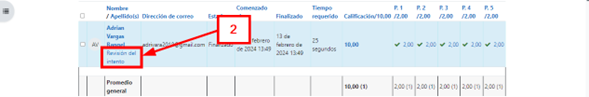
\includegraphics[width=0.9\linewidth]{include/moodle_step2.png}
    \caption{Revisión del intento}
    \label{fig:nasa-tlx-propio}
\end{figure}

A continuación, se describe el proceso de uso del script de webscrapping para la extracción y cálculo de los tiempos de respuesta:

\begin{enumerate}
    \item Descargar Python 3.12.0 o superior
    \item Descargar la carpeta \texttt{web\_scraping\_response\_times}
    \item Guardar como html la revisión del intento de cada participante dentro de la carpeta descargada
    \item Abrir una terminal en la carpeta descargada
    \item Ejecutar la línea: \texttt{python extractor.py}
    \item Se creará el archivo de Excel “\texttt{all\_response\_times}” con los tiempos de respuesta calculados en segundos
\end{enumerate}



Las pruebas con las preguntas dummy confirmaron que el sistema de Moodle puede ser utilizado con el script de webscrapping adjunto en el repositorio de github de esta memoria para extraer la hora de inicio y fin de cada pregunta del cuestionario y calcular el tiempo de respuesta del participante, lo que facilita la futura implementación del cuestionario completo.

\begin{figure}[h]
    \centering
    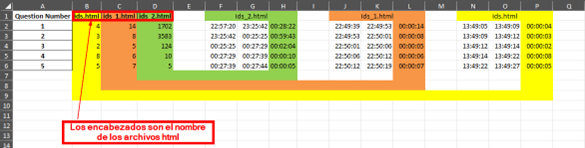
\includegraphics[width=0.9\linewidth]{include/resultados_excel.png}
    \caption{EJemplo de registro de tiempo de respuesta por pregunta. Cada columna de B a D representa el cuestionario de un participante individual}
    \label{fig:nasa-tlx-propio}
\end{figure}




Este proceso asegura que el cuestionario pueda ser desplegado en el entorno de Moodle de la universidad en futuras implementaciones, proporcionando una herramienta adecuada para evaluar la interpretabilidad de los modelos de inteligencia artificial.





 